\chapter{Testes de carga}
\label{chap:testes}

\hspace{5mm} Em qualquer sistema, após a criação e configuração do deployment automatizado é necessário efectuar \textbf{testes de carga} antes da produção, desta forma o grupo criou \textbf{6 casos de testes}.

\hspace{5mm} Foram testados os métodos login e create apenas no serviço do Personal Trainer \textbf{inferindo-se que o desempenho dos mesmos seriam idênticos} no serviço Client pois realizam lógica idêntica.

\hspace{5mm} \textbf{Note-se que o grupo tem consciência que caso este projecto fosse em ambiente profissional e realmente fosse para entrar em produção todos os micro-serviços seriam testados individualmente, inclusive com várias configurações dos recursos das máquinas utilizadas e da infraestrutura. No entanto, visto que o ambiente é académico e os testes de carga não são o principal objectivo de avaliação, decidiu-se simplificar os mesmos.}

\hspace{5mm} Para a execução dos testes utilizou-se a ferramenta \href{https://jmeter.apache.org}{apache jmeter} sendo esta escolhida porque o grupo já estava familiarizado com a mesma uma vez que a utilizou noutros projectos.

\hspace{5mm} Para a \textbf{automatização dos testes}, primeiramente foram definidos os 6 testes de carga e guardadas as suas configurações nos ficheiros \textbf{.jmx}. De seguida foram adicionadas opções num Makefile que executam os testes \textbf{individualmente ou todos sequencialmente} tal como a seguinte figura sugere.

\begin{figure}[H]
    \centering
    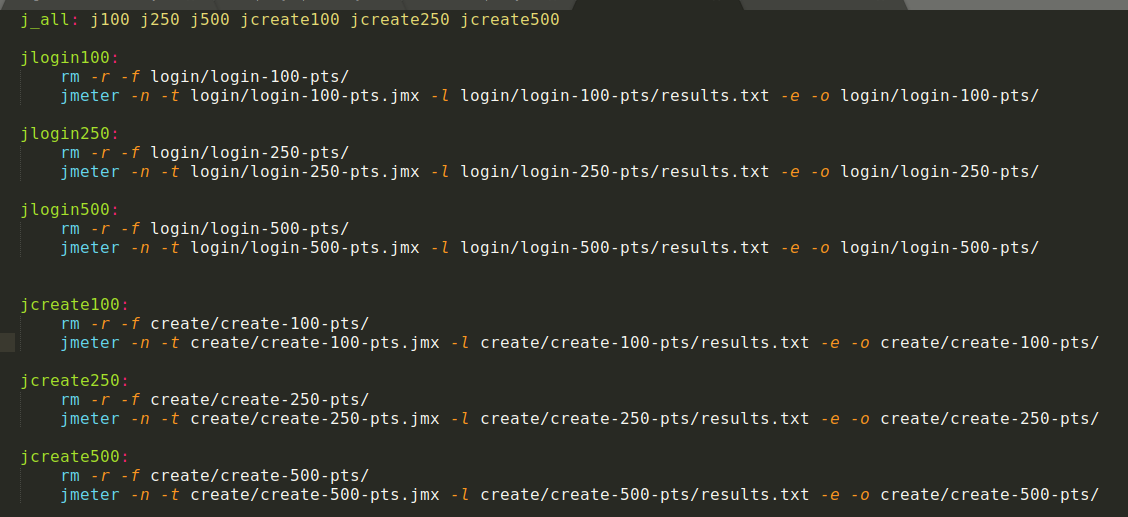
\includegraphics[scale=0.4]{images/jmeter.png}
    \caption{Makefile para automatização dos testes de carga.}
    \label{fig:makefile}
\end{figure}

\hspace{5mm} Tal como se pode observar na figura o micro-serviços foram testados para \textbf{100, 250 e 500 personal trainers}. Todos os resultados obtidos serão colocados em anexo, no entanto nesta secção apenas serão abordados os resultados para 500 clientes.

\hspace{5mm} Os métodos testados  foram o \textbf{HTTP POST /PersonalTrainer/api/login} e o \textbf{HTTP POST /PersonalTrainer/api/createPersonalTrainer}. O conteúdo json enviado para cada um foi previamente calculado (no povoamento automático da base de dados) e de modo a simular a utilização real do sistema cada thread do jmeter (que representa um personal trainer a aceder ao sistema) contém um json específico que se encontra num ficheiro pts-data.csv.


\subsection{login para 500 Personal Trainers}

\hspace{5mm} Os dados obtidos para o teste do login para 500 Personal Trainers foram os seguintes.

\begin{figure}[H]
    \centering
    \includegraphics[scale=0.45]{images/login-500-pts.png}
    \caption{login para 500 Personal Trainers}
    \label{fig:login500}
\end{figure}

\hspace{5mm} \textbf{Note-se que o valor máximo para o tempo de resposta foi um pedido que demorou 5601 ms a ser processado, no entanto pode ser considerado um \href{https://en.wikipedia.org/wiki/Outlier}{outlier} uma vez que o percentil 99th indica que 99\% dos pedidos foram processados em menos de 765.75 ms, sendo um tempo de resposta útil.}